\section{Sampling methods}
\label{sampling_methods}

According to the theory of the Diffusion approximation and the BSSRDF model, SSS light
contribution at each point of the surface of the object depends on the irradiance over the full area
of the object. Thus, strictly speaking, it requires the integration along the area of the whole
object.
\[
L_o(x_o, \vec{\omega_o})= \int_{A} R_d(x_i-x_o) \Bigg[ \int_{\Omega}
L_i(x_i,\vec{\omega_i})d\omega_i \Bigg] dA(x_i)
\]

This simplified formulation of the light equation using BSSRDF model is indeed a double integral.
The inner integral over the hemisphere stands for gathering of the light contribution at each point
of the object. Efficient sampling of that term is one of the fundamental topics in computer
graphics. It is common problem both for rendering solid objects with BRDF approximation or SSS media
with BSSRDF model. And it is not discussed here.

The outer integral over the area, on the other hand, is a definitive part of the BSSRDF formulation.
At each sample of this the area integration the inner integral over the hemisphere has to be
calculated. This fact substantially increases complexity of the light integration and make is
especially important to optimize the area sampling.

The fast fade out of BSSRF functions with distance allows in practice to avoid the integration over
the whole object. Usually, only the local area around the shading position is integrated with
preserving considerable accuracy of the final result. The practical details of area sampling are
described in the following sections.

\subsection{Infinite plane disk sampling}
\label{subsection:sampling_simple_disk}
The planar geometry assumption, described in the section \ref{section:BSSRDF_intuition} about the
basics of the BSSRDF and section \ref{section:searchlight} about the  Searchlight experiment, makes
it trivial to sample the area around the shading point to integrate SSS light contribution.
\begin{wrapfigure}{r}{0.3\textwidth}
    \begin{center}
        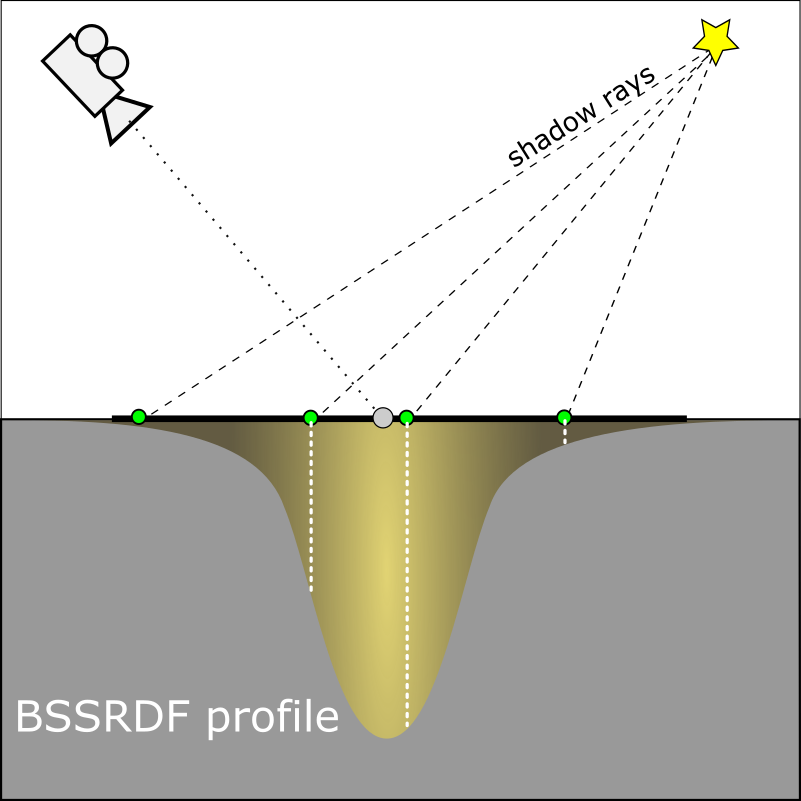
\includegraphics[width=0.29\textwidth]{schemes/sampling_naive_plane}
        \caption{The naive disk sampling}
    \end{center}
    \vspace{5pt}
    \label{fig:sampling_naive}
\end{wrapfigure}
\begin{wrapfigure}{r}{0.3\textwidth}
    \begin{center}
        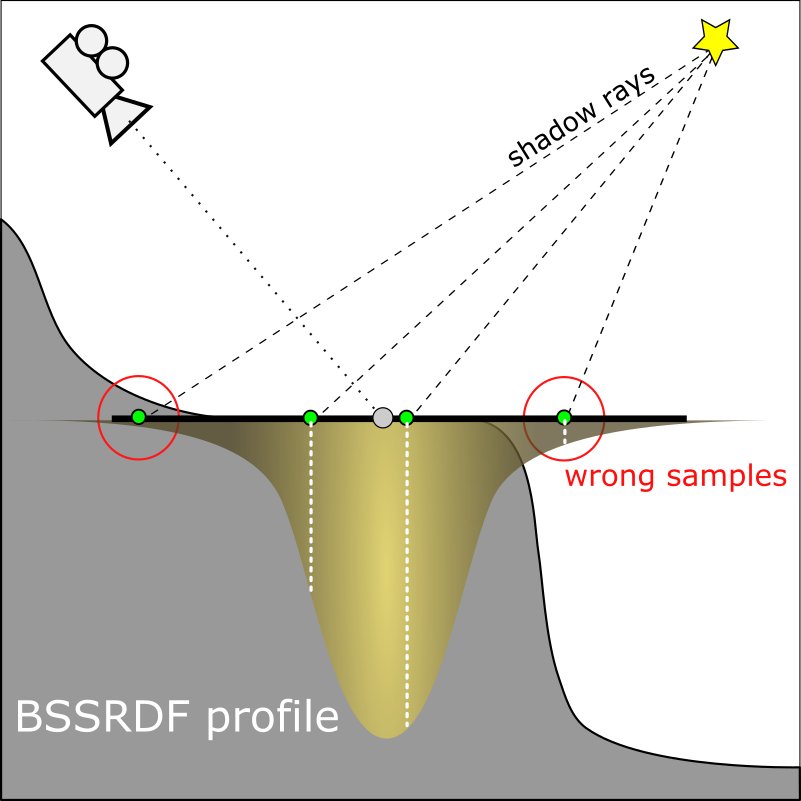
\includegraphics[width=0.29\textwidth]{schemes/sampling_naive_failing}
        \caption{Naive disk sampling fails on curved geometry}
    \end{center}
    \vspace{-20pt}
    \label{fig:sampling_naive_fails}
\end{wrapfigure}
Classic approach of integrating the BSSRDF described by \cite{Jensen:2001:PMS:383259.383319} 
produce very good approximation in the case of locally flat geometry. The approach is based on the
sampling of the area of the disk located with it's center in the current shading point and oriented
by normal to the surface. The naive approach would utilize the uniform distribution of samples over
the area of the disk.

The light contribution $L$ is estimated by tracing the shadow ray to the light source and
weighted by the BSSRDF value taking into account the distance $r$ between center of the disk and
sampling position. This sampling technique produce very good approximation in case of the flat
infinite plane. But fails in any case of non-planar geometry.

A number of sampling techniques where proposed in the literature to improve handling of complex
geometries. Such as Multiresolution radiosity caching \cite{Christensen:2012:MRC:2343045.2343108} or
Bidirectional Lightcuts \cite{Walter:2012:BL:2185520.2185555}. But yet non of them are robust enough
to integrate the BSSRDF on models with high curvatures with good accuracy.

\subsection{Multiple disks sampling}
Multiple disks sampling is one of the popular methods used by several production tools. It was first
described by \cite{King:2013:BIS:2504459.2504520}. And can be seen as an extension of the classic
disk sampling method described in section \ref{subsection:sampling_simple_disk}.
\begin{figure}[h]
    \centering
    \begin{subfigure}{0.45\textwidth}
        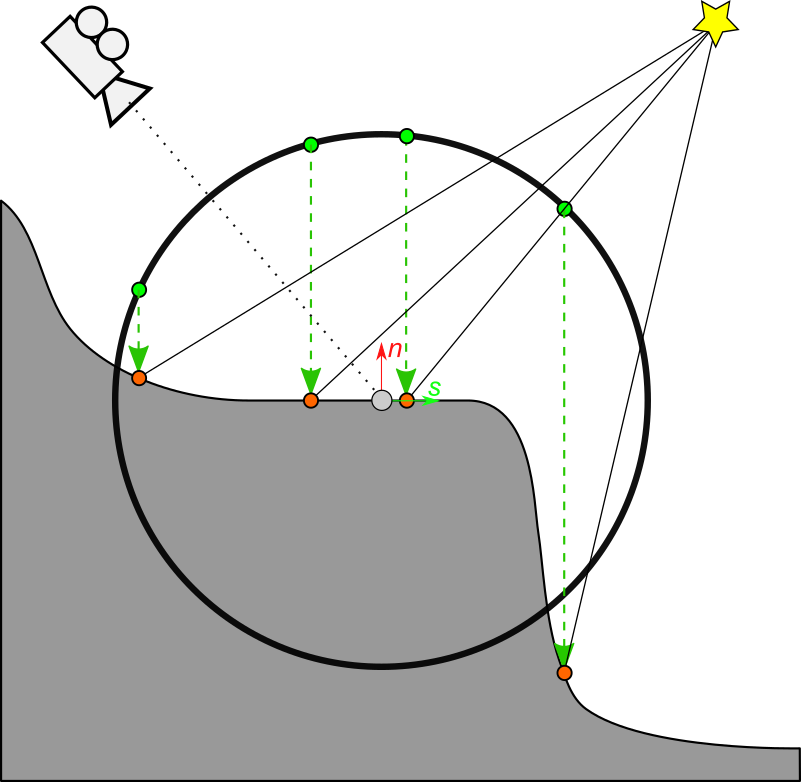
\includegraphics[width=\textwidth]{schemes/sampling_rays}
        \caption{Sampling along normal direction $\vec{n}$}
        \label{fig:sampling_rays_n}
    \end{subfigure}
    \quad
    \begin{subfigure}{0.45\textwidth}
        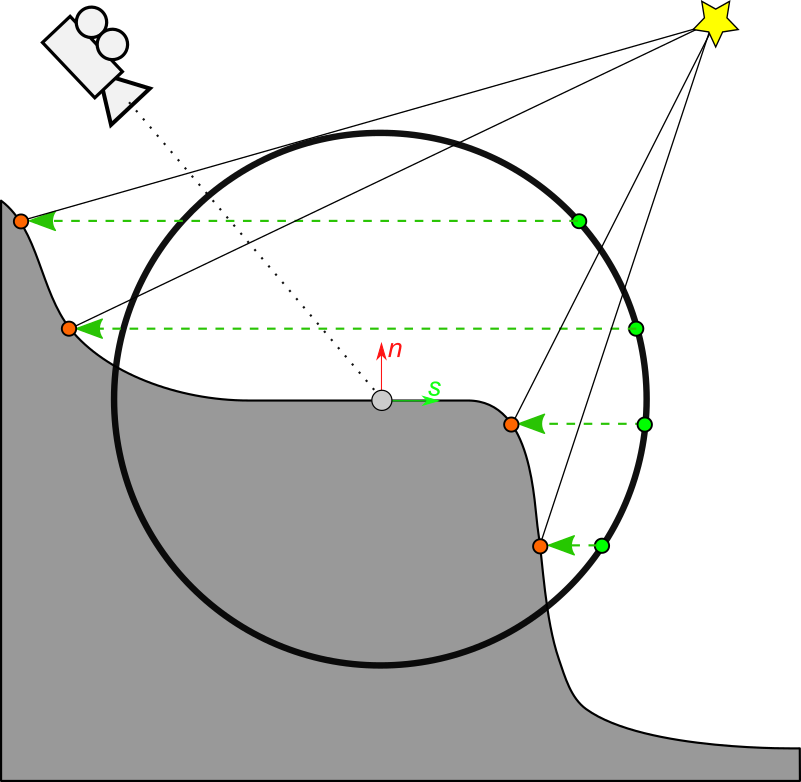
\includegraphics[width=\textwidth]{schemes/sampling_rays_side}
        \caption{Sampling along tangent direction $\vec{s}$}
    \end{subfigure}
    \caption{Samples are projected to the sphere. Ray tracing is done along 3 principal axes}
    \label{fig:sampling_rays}
\end{figure}

First improvement is introduced by finding the actual point on the geometry instead of preforming
shadow tests from the virtual disk surface. Simple way to find these positions on the geometry is by
casting a short rays with the origins at the disk, shifted along the shading normal.
The direction of the local rays is negative to the shading normal.

More robust approach is to project the samples from the disk to the the surface of a virtual sphere
around the shading position. The ray tracing is preformed the same way in the negative normal
direction \ref{fig:sampling_rays_n}.

This ray tracing procedure indeed increases the computation time of the BSSRDF sampling. But the
modern ray tracing engines allow to preform efficient ray-geometry intersection tests for short rays
with locally bounded geometries by using efficient acceleration data structures. The fact, that
there is no need to traverse the whole scene also greatly improves the performance of such sampling.

The next step in increasing robustness of the disk sampling is done by making three disk samples
instead of one. The axes of each of the the disk are aligned along the local orthonormal basis
vectors $(\vec{n},\vec{s},\vec{t})$ of the geometry in the point of shading.
According to \cite{King:2013:BIS:2504459.2504520}, the usual normal aligned disk is weighted with
0.5 probability. The $s$ and $t$ aligned disk samples have 0.25 contribution. The multiple
importance sampling combination of this this three disk samples allows to greatly increase the
performance of the BSSRDF integration.